\documentclass{standalone}
\usepackage{xcolor}
\usepackage{verbatim}
\usepackage[T1]{fontenc}
\usepackage{graphics}
\usepackage{hyperref}
\newcommand{\code}[1]{\texttt{#1}}
\newcommand{\R}{R}
\newcommand{\pkg}[1]{#1}
\newcommand{\CRANpkg}[1]{\pkg{#1}}%
\newcommand{\BIOpkg}[1]{\pkg{#1}}
\usepackage{amsmath,amssymb,array}
\usepackage{booktabs}
\usepackage{multicol, calc}
\usepackage{tikz}
\usetikzlibrary{patterns,positioning,babel}
\usepackage{threeparttable}
\usepackage{natbib}
\usepackage{inconsolata}
\usepackage{listings}
\usepackage{tikz-qtree}
\usepackage{subcaption} 

\begin{document}
\nopagecolor
	
		
		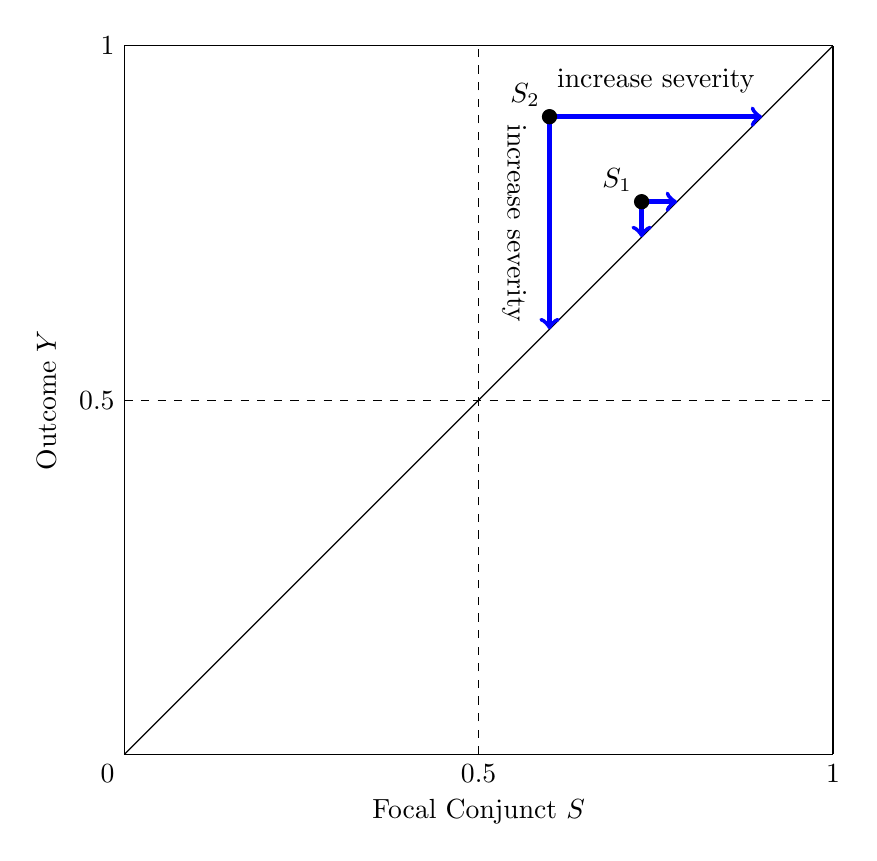
\begin{tikzpicture}[scale=9]
		\draw[black] (0,0) -- (1,0) node at (0.5,-0.08){Focal Conjunct $S$};
		\draw[black] (0,0) -- (0,1) node at (-0.11,0.5)[rotate=90] {Outcome $Y$};
		\draw[black] (0,0) -- (1,1);
		\draw[black] (0,1) -- (1,1);
		\draw[black] (1,0) -- (1,1);
		\draw[dashed] (0.5,0) -- (0.5, 1);
		\draw[dashed] (0,0.5) -- (1, 0.5);
		\draw[->, ultra thick, blue] (0.73, 0.78) -- (0.78, 0.78) ;
		\draw[->, ultra thick, blue] (0.73, 0.78) -- (0.73, 0.73) ;
		\draw[fill] (0.73,0.78) circle [radius=0.01] node [above left] {$S_1$};
		\draw[->, ultra thick, blue] (0.6,0.9) -- (0.9,0.9) ;
		\draw[->, ultra thick, blue] (0.6,0.9) -- (0.6,0.6);
		\draw[fill] (0.6,0.9) circle [radius=0.01] node [above left] {$S_2$};
		\node at (0.75,0.95){increase severity};
		\node [rotate=-90] at (0.55,0.75){increase severity};
		\node [below left] at (0,0){$0$};
		\node [left] at (0,1){$1$};
		\node [below] at (1,0){$1$};
		\node [left] at (0,0.5){$0.5$};
		\node [below] at (0.5,0){$0.5$};
		\end{tikzpicture}
		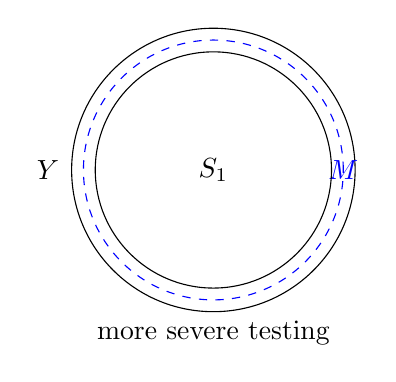
\begin{tikzpicture}[scale=3]
		\draw (3,0.5) circle [radius=0.6] node at (2.3,0.5){$Y$};
		\draw[dashed, blue] (3,0.5) circle [radius=0.55] node at (3.55,0.5){$M$};
		\draw (3,0.5) circle [radius=0.5] node at (3,0.5){$S_1$};
		\node [above] at (3,-0.28){more severe testing};
		\end{tikzpicture}
		\qquad
		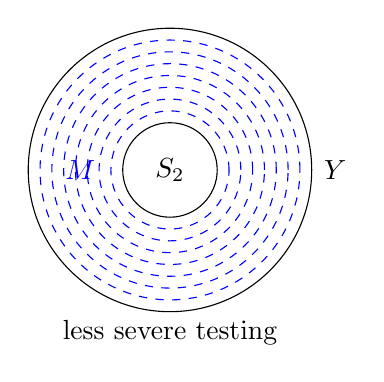
\begin{tikzpicture}[scale=3]
		\draw (3,0.5) circle [radius=0.6] node at (3.7,0.5){$Y$};
		\draw[dashed, blue] (3,0.5) circle [radius=0.55];
		\draw[dashed, blue] (3,0.5) circle [radius=0.5];
		\draw[dashed, blue] (3,0.5) circle [radius=0.45];
		\draw[dashed, blue] (3,0.5) circle [radius=0.4] node at (2.62,0.5){$M$};
		\draw[dashed, blue] (3,0.5) circle [radius=0.35];
		\draw[dashed, blue] (3,0.5) circle [radius=0.3];
		\draw[dashed, blue] (3,0.5) circle [radius=0.25];
		\draw (3,0.5) circle [radius=0.2] node at (3,0.5){$S_2$};
		\node [above] at (3,-0.28){less severe testing};
		\end{tikzpicture}
\end{document}
